\section{Single player flowchart and explanation~\ref{fig:singleplayer}}

\begin{figure}
    \centering 
    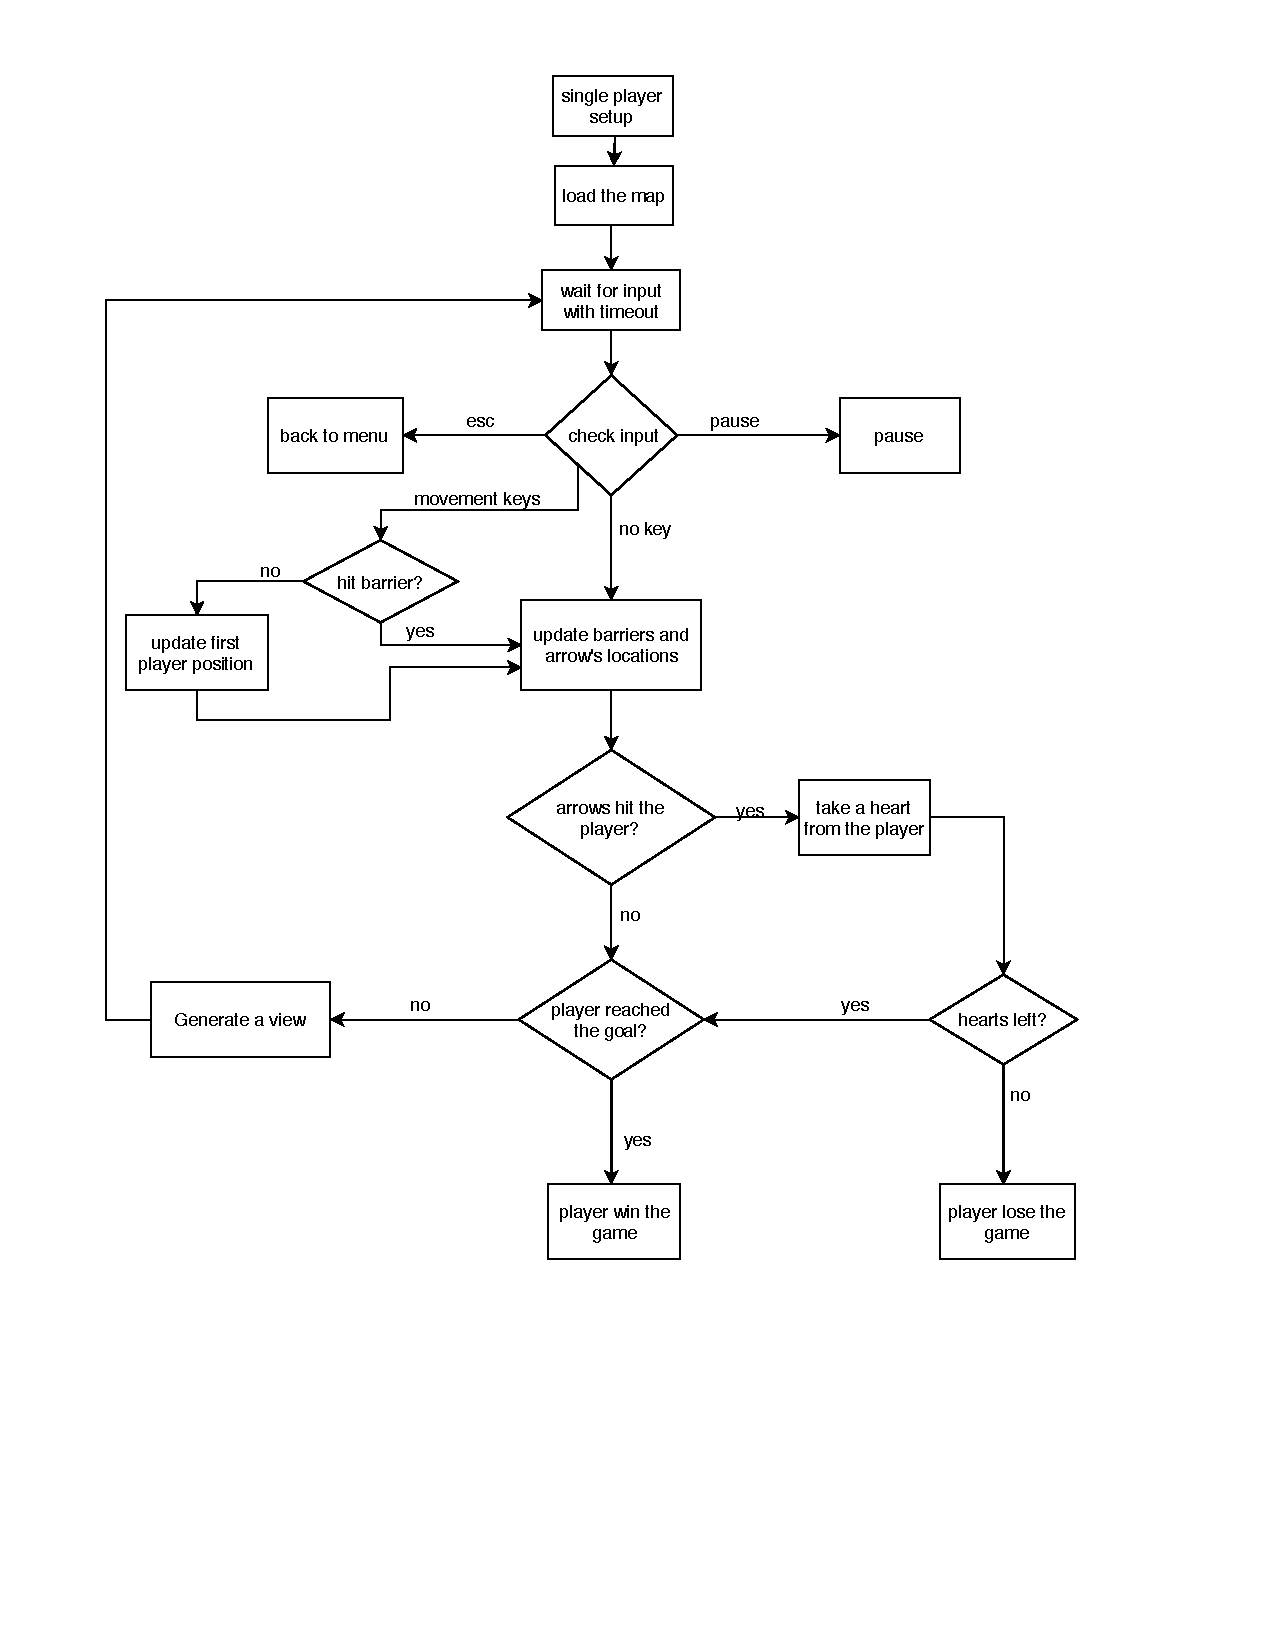
\includegraphics[width=\columnwidth]{singleplayer.pdf}
    \caption{Single player block flowchart. white blocks will be implemented in the first release.}
    \label{fig:singleplayer}
\end{figure}

This flow chart explains all the steps happening on single player mode. 
As it is shown in Figure~\ref{fig:singleplayer}, load the map block reads the map from a text file. Next, we do some setups for single player game based on the map. In these setups we define a map with position of the player, the goal, the barriers and the arrows.
We should then read the input keyboard buffer and wait for input. The reading process is done within a limited time and there exist a timeout which expires if no input is provided within that time. Then the program checks the input to see what key has entered. If pause button is entered, program goes to pause game state. If escape button is pressed, program goes to menu. If no keys has entered, program updates the position of barriers and arrows as they are moving objects. If entered keys are movement keys, program first check if the player's move is permitted or not (checks map walls and barriers); if yes, then program updates the player position, barriers and arrows locations, and checks if the player is hit. If player can not move, program only updates barriers and arrows and does not change player's location. If player is hit by an arrow, it loses one heart and immediately checks if there is any heart left for the player. If the player loses all of its hearts, player loses the game. If the player has still a heart, program check if the player reaches the goal. Player wins the game if it reach the goal, otherwise program \textcolor{blue}{\bf generate a view} to display any updates on the map. Then wait for input key and it will continue until the player wins or loses the game.
The graphic part of the game is done using SDL library. The logic of the game is independent of graphics.

\subsection{Single player functions prototypes}
In this section we define the required functions prototypes and its relation to flow chart~\ref{fig:singleplayer}. We define some functions and the rest of the code will be in a main function. Comments above each function mention the associated block, the release, and assignee.

\begin{minted}{c}
#define MAP_MAX_NUM_OF_BARRIERS 10
#define MAP_MAX_NUM_OF_ARROWS 20
#define MAP_MAX_NUM_OF_PLAYERS 2
#define BARRIER_MOVE_STEP_SIZE 1
#define ARROW_MOVE_STEP_SIZE(speed) (((speed)+1)*2)
#define PLAYER_MOVE_STEP_SIZE 10
#define BULLET_MOVE_STEP_SIZE 6
#define MAP_MAX_NUM_OF_BULLETS 2

 /**
  * @typedef position_t
  * A structure represents the position.
  */
typedef struct position {
	int x;             /**< position in x coordinate */
	int y;             /**< position in y coordinate */
} position_t;

/**
 * @typedef direction_t
 * The enumeration of movement direction.
 */
typedef enum direction {
	DIRECTION_RIGHT,
	DIRECTION_LEFT,
	DIRECTION_UP,
	DIRECTION_DOWN
} direction_t;

/**
 * @typedef player_index_t
 * The enumeration of player.
 */
typedef enum player_index {
	PLAYER_1,
	PLAYER_2,
} player_index_t;


/**
 * @typedef map_space_t
 * A structure represents the space which map is defined in it.
 */
typedef struct map_space {
	int x_min;
	int x_max;
	int y_min;
	int y_max;
} map_space_t;

/**
 * @typedef map_barrier_t
 * A structure represents the a barrier in the map.
 */
typedef struct map_barrier {
	position_t current_pos;     /**< current position of a barrier*/
	int length;                 /**< length of a barrier*/
	direction_t current_dir;    /**< current direction of a barrier*/
} map_barrier_t;

/**
 * @typedef arrow_t
 * A structure represents an arrow in the map
 */
typedef struct arrow {
	position_t current_pos;    /**< current position of an arrow*/
	int speed;                 /**< the speed of an arrow*/
	direction_t direction;     /**< direction of an arrow*/
} arrow_t;


/**
 * @typedef bullet_t
 * A structure represents a bullet in the map
 */
typedef struct bullet {
	position_t current_pos;    /**< current position of a bullet*/
	int speed;                 /**< the speed of a bullet*/
	direction_t direction;     /**< direction of a bullet*/
} bullet_t;


/**
 * @typedef player_t
 * A structure represents a player in the map
 */
typedef struct player {
	position_t current_pos;    /**< current position of the player*/
	int heart;                 /**< number of the heart the player have*/
	bullet_t bullet;           /**< bullet generated from player*/
	bool bullet_is_active;     /**< defines if the bullet is inside the map space or not*/
} player_t;


/**
 * @typedef goal_t
 * A structure represents the goal in the map
 */
typedef struct goal {
	position_t pos;         /**< position of the goal in the map*/
} goal_t;

/**
 * @typedef map_textures_t
 * A structure represents the single player map's textures.
 */
typedef struct map_textures {
	SDL_Texture* p_texture_player[MAP_MAX_NUM_OF_PLAYERS];
	SDL_Texture* p_texture_heart[MAP_MAX_NUM_OF_PLAYERS];
	SDL_Texture* p_texture_goal;
	SDL_Texture* p_texture_arrow_down;
	SDL_Texture* p_texture_arrow_up;
	SDL_Texture* p_texture_barrier;
} map_textures_t;

/**
 * @typedef map_textures_multi_t
 * A structure represents the multi player map's textures.
 */
typedef struct map_textures_multi {
	SDL_Texture* p_texture_player;
	SDL_Texture* p_texture_heart;
	SDL_Texture* p_texture_player_1;
	SDL_Texture* p_texture_heart_1;
	SDL_Texture* p_texture_goal;
	SDL_Texture* p_texture_arrow_down;
	SDL_Texture* p_texture_arrow_up;
	SDL_Texture* p_texture_barrier;
	SDL_Texture* p_textture_bullet;
} map_textures_multi_t;


/**
 * @typedef map_t
 * A structure represents the map entities
 */
typedef struct map {
	map_space_t space;          /**< space of the map*/
	int number_of_barriers;     /**< number of barriers in the map*/
	int number_of_arrows;       /**< number of arrows in the map*/
	int number_of_players;      /**< number of players in the map*/
	map_barrier_t barrier[MAP_MAX_NUM_OF_BARRIERS]; /**< barries in the map*/
	arrow_t arrow[MAP_MAX_NUM_OF_ARROWS];   /**< arrows in the map*/
	goal_t goal;                            /**< goal in the map*/
	player_t player[MAP_MAX_NUM_OF_PLAYERS];/**< player in the map*/
	map_textures_t textures;                /**< single player map's element textures*/
	map_textures_multi_t textures1;         /**< multi player map's element textures*/
} map_t;

/**
 * @brief loads the map.
 * @author Pari
 * Wrote for release one and updated for release two.
 * This function parses the map file and initializes the map structure using input file.
 * @param [in] file_path input file path.
 * @return filled map structure.
 */
map_t load_map(char* file_path);

#define MAP_TEXTURE_PLAYER_WIDTH 30
#define MAP_TEXTURE_PLAYER_HEIGHT 30
#define MAP_TEXTURE_HEART_WIDTH 25
#define MAP_TEXTURE_HEART_HEIGHT 25
#define MAP_TEXTURE_GOAL_WIDTH 30
#define MAP_TEXTURE_GOAL_HEIGHT 30
#define MAP_TEXTURE_ARROW_WIDTH 10
#define MAP_TEXTURE_ARROW_HEIGHT 40
#define MAP_TEXTURE_BARRIER_HEIGHT 3
#define MAP_TEXTURE_BARRIER_WIDTH_MAX 400
#define MAP_TEXTURE_BULLET_WIDTH 15
#define MAP_TEXTURE_BULLET_HEIGHT 15


/**
 * @brief creats player texture.
 * @author Pari
 * Wrote for release one and updated for release two.
 * @param[in] p_renderer
 * @param[in] player_index
 * @return p_texture player texture
 */
static inline SDL_Texture* get_player_texture(SDL_Renderer* p_renderer,
                                              player_index_t player_index);

/**
 * @brief creats heart texture for each player.
 * @author Jin
 * Release one
 * @param[in] p_renderer
 * @param[in] player_index
 * @return p_texture heart texture
 */
static inline SDL_Texture* get_heart_texture(SDL_Renderer* p_renderer,
                                             player_index_t player_index);

/**
 * @brief creats goal texture.
 * @author Pari
 * Release one
 * @param[in] p_renderer
 * @return p_texture goal texture
 */
static inline SDL_Texture* get_goal_texture(SDL_Renderer* p_renderer);

/**
 * @brief creats arrow down texture.
 * @author Pari
 * Release one.
 * @param[in] p_renderer
 * @return p_texture arrow down texture
 */
static inline SDL_Texture* get_arrow_down_texture(SDL_Renderer* p_renderer);

/**
 * @brief creats arrow up texture.
 * @author Pari
 * Release one.
 * @param[in] p_renderer
 * @return p_texture arrow up texture
 */
static inline SDL_Texture* get_arrow_up_texture(SDL_Renderer* p_renderer);

/**
 * @brief creats barrier texture.
 * @author Pari
 * Release one.
 * @param[in] p_renderer
 * @param[in] length of barrier, is read from map file.
 * @return p_texture barrier texture
 */
static inline SDL_Texture* get_barrier_texture(SDL_Renderer* p_renderer, int length);

/**
 * @brief creats bullet texture.
 * @author Mahsa
 * Release two
 * @param[in] p_renderer
 * @return p_texture bullet texture
 */
static inline SDL_Texture* get_bullet_texture(SDL_Renderer* p_renderer);

/**
 * @brief game_state_t enumeration of game states
 */
typedef enum game_state {
    GAME_STATE_UNDEFINED,
    GAME_STATE_RUN,
    GAME_STATE_PAUSE,
    GAME_STATE_LOSE,
    GAME_STATE_WIN,
} game_state_t;

/**
 * @brief game over function
 * @author Pari
 * Release one
 * This function clears the renderer and shows a texture (game over) on the window.
 * @param [in] p_window the same window is used to display win game text.
 * @return void
 */
void game_over(SDL_Window* p_window);

/**
 * @brief win game function
 * @author Pari
 * Release one
 * This function clears the renderer and shows a texture (win game) on the window.
 * @param [in] p_window the same window is used to display win game text .
 * @return void
 */
void win_game(SDL_Window* p_window);

/**
 * @brief Checks if a player is hit by arrows.
 * @author Pari
 * Release one
 * This function checks if a player is hit by arrows.
 * @param [in] map represents map's structure which has player, arrows, ...info.
 * @param [in] player_index  can be PLAYER1 or PLAYER2.
 * @return flag if the player is hit, flag = 1, otherwise flag = 0.
 */
int is_player_hit(map_t* map, player_index_t player_index);

/**
 * @brief check the collision
 * @author Mahsa
 * Release one
 * This function get player's position and checks if it hits any of the barriers/borders.
 * NOTE: The border of the map also be considered as barrier.
 * @param[in] map  map structure represents players, barriers, and... position.
 * @param[in] direction specify player's next movement.
 * @param[in] player_index specify the player: PLAYER_1/PLAYER_2.
 * @return bool true if player hit a barrier or borders and false otherwise.
 */
bool is_barrier_hit(map_t map, direction_t direction, player_index_t player_index);

/**
 * @brief update the position of the player
 * @author Mahsa
 * Release one
 * This function gets the direction in which the player wants to move as well as the player
 * itself and updates the player's position based on the direction.
 * NOTE: This function only be called after validation of the player's move;
 * @param[in] player information of the player: position, ... .
 * @param[in] direction player's movement direction.
 * @param[out] player's position will be updated.
 */
void update_player_pos(player_t* player, direction_t direction);

/**
* @brief generate_view function
* @author Jin
* Release one
* This function is to generate a graphic map using updated information
* @param[in] p_window a SDL window which is passed from the main function.
* @param[in] p_map a defined map which is passed from the main function.
* @return void
*/
void generate_view(SDL_Window* p_window, map_t* p_map);

/**
 * @brief Checks if the player reached the goal
 * @author Wrote by Jaser updated by Pari
 * Release one
 * @param[in] p_player player information including position.
 * @param[in] p_goal goal's position
 * @return false if the player does not reach the goal and true otherwise.
 */
bool is_reach_goal(player_t* p_player, goal_t* p_goal);

/**
 * @brief This function is to update barrier position in the map.
 * @author Wrote by Jin
 * Release one
 * @param[in] barrier a pointer to access to each barrier
 * stored in a map_barrier structure array.
 * @param[in] map represents the map structure including borders,... .
 * @param[out] update barrier's position.
 */
void update_barrier(map_barrier_t* p_barrier, map_t* map);

/**
 * @brief This function is to update arrow position in the map.
 * @author Wrote by Jaser updated by Pari
 * Release one
 * @param[in] arrow a pointer to access to each arrow stored in a arrow structure array.
 * @param[in] map represents map's structure.
 * @param[out] update arrow's position.
 */
void update_arrow(arrow_t* p_arrow, map_t* map);

/**
 * @brief This function is to take a heart from the player.
 * @author Jin
 * Release one
 * @param[in] player a structure represents the player: position, heart, ....
 */
void take_heart(player_t* p_player);
\end{minted}